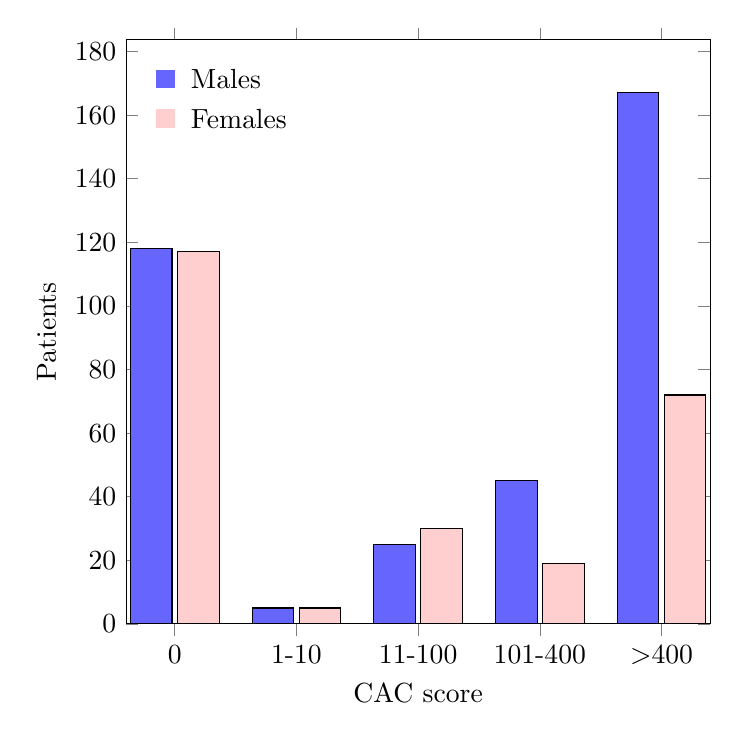
\begin{tikzpicture}
    \begin{axis}[
        name=cac_by_gender,height=9cm,width=9cm,
        % title={CAC score by gender distribution},
        ybar,
        symbolic x coords={0, 1-10, 11-100, 101-400, $>$400},
        ymin=0,ylabel={Patients},
        xmin=0,xtick=data,xlabel={CAC score},
        bar width=15pt,
        enlarge x limits=0.1,
        % nodes near coords={\pgfmathprintnumber\pgfplotspointmeta} % put value on bar top
    ]
        \addplot[fill=blue!60] coordinates {
            (0,118)
            (1-10,5)
            (11-100,25)
            (101-400,45)
            ($>$400,167)
        };
        \addplot[fill=pink!75] coordinates {
            (0,117)
            (1-10,5)
            (11-100,30)
            (101-400,19)
            ($>$400,72)
        };
    \end{axis}
    \node[fill=blue!60,xshift=0.5cm,yshift=-0.5cm] at (cac_by_gender.north west) (male) {};
    \node[right of=male,anchor=west,xshift=-0.8cm] {Males};
    \node[fill=pink!75,below of=male,yshift=0.5cm] (female) {};
    \node[right of=female,anchor=west,xshift=-0.8cm] {Females};
\end{tikzpicture}
